\section{研究问题与 OpenMAIC 机制}
本章检验角色分工、可执行证据和持久学习记录，能否把能力有限的教育语言模型组织成可核验的教学流程。评价区分完整系统与模型本身：成功检索历史或给出正确回退答案，不等于模型已经能够自主教学。研究问题分别涉及调度机制、跨轮学生证据，以及教学请求成功或失败的具体原因。

源码分析固定于 OpenMAIC 官方提交 \texttt{5bd8cc840ee63}，检索日期为2026年11月6日\cite{openmaic}。完整提交号、永久链接与19份归档文件的 SHA-256 见 \path{tutor/legacy/research/source_manifest.json}。本项目没有部署原 OpenMAIC；后续 Python 系统是独立简化实现，主要借鉴表\ref{tab:concise-agents-source}中的四类机制。

\begin{table}[htbp]\centering\small
\caption{OpenMAIC 的实际机制与固定源码锚点。表内路径相对固定的上游仓库，永久链接保留于来源清单。}\label{tab:concise-agents-source}
\begin{tabularx}{\linewidth}{@{}p{25mm}Yp{65mm}@{}}\toprule
机制 & 源码实际实现 & 来源位置\\\midrule
角色与调度 & 教师、助教、同学具有不同提示和动作；Director 用 \texttt{call\_agent} 选择有用的发言者，并非固定轮流。子角色可共享模型对象；结束动作检查是否已有可见回应或实质教学内容。 & \path{registry/built-in.ts}:12--155；\path{pi/director-loop.ts}:95--221；\path{pi/tools/call-agent.ts}:735--757、847--864。\\
课程状态与证据 & 材料分析、资料研究先于大纲和场景生成；完成步骤是显式状态。\texttt{read\_scene} 向后续角色提供页面证据，限制无依据猜测。 & \path{generation/run/plan.ts}:45--103；\path{generation/src/scene-builder.ts}:21--116；\path{pi/tools/read-scene.ts}:97--124。\\
上下文与记忆 & 子角色保留最近12条消息；Director 压缩时保留目标与未解决问题。PBL Instructor 在历史超过30条后向最近16条压缩，提取学习线索并读回 \texttt{earlierSummary}；摘要压缩阈值为4500字符。 & \path{pi/prompts.ts}:558--589；\path{pi/director-compaction.ts}:95--101、136--217；\path{v2/agents/instructor-memory.ts}:22--138。\\
反馈与回退 & 测验区分提交前后状态，提交后的学生答案、参考、评分和评语用于反馈。模型评分无法解析时可回退半分；这维持接口运行，并不能证明答案正确。 & \path{summarizers/state-context.ts}:172--240；\path{api/quiz-grade/route.ts}:56--105。\\\bottomrule
\end{tabularx}
\end{table}\FloatBarrier

因此，OpenMAIC 不只有聊天历史，还包含场景状态与显式学习者摘要；但由关键词提取的进度线索不等于经过核验的掌握度。本项目保留分工、共享证据和显式控制，将多媒体课堂缩小为可执行的 Python 输出题，不复现语音、白板和完整课程编辑器。

\section{实现与可核验学生记忆}
控制器顺序调用规划、教学、评审角色，三者共享一次加载的模型。原版使用第二章 SFT；后续分别接入真实云端 SFT 检查点和明确区分的官方 Instruct 模型，本章不更新权重。规划返回关注点和策略；教学返回答案、反馈、解释及可选 \texttt{followup\_code}；评审返回 \texttt{approved} 和理由。实际提示为中文；完整模板、逐次上下文、原始回应、token 编号、停止原因和采用决定均留档。

受限 AST 解释器计算输出与轨迹，不把生成文本交给无限制的 \texttt{eval}/\texttt{exec}。评估器另用 CPython 执行已审阅、冻结的参考程序；不支持的程序不能直接取得参考答案并冒充已核验。原版采用门槛检查答案、必需解释/反馈文本、评审批准及复测可执行性；修订控制器才增加学生状态、事实证据和明确变式修改约束，历史C08运行尚无这些较强检查。这不能证明全部自然语言解释。被拒草稿保留，最终回答明确标注工具或模板回退来源。

原版在本机 CPU 上以 float32、六线程和贪心解码运行，每角色最多生成256个新 token；输入与生成合计超过4096时明确报错，不静默截断。修订角色预算为64/192/96。各组分别冻结实现、模型、提示和预算。

\begin{figure}[htbp]\centering
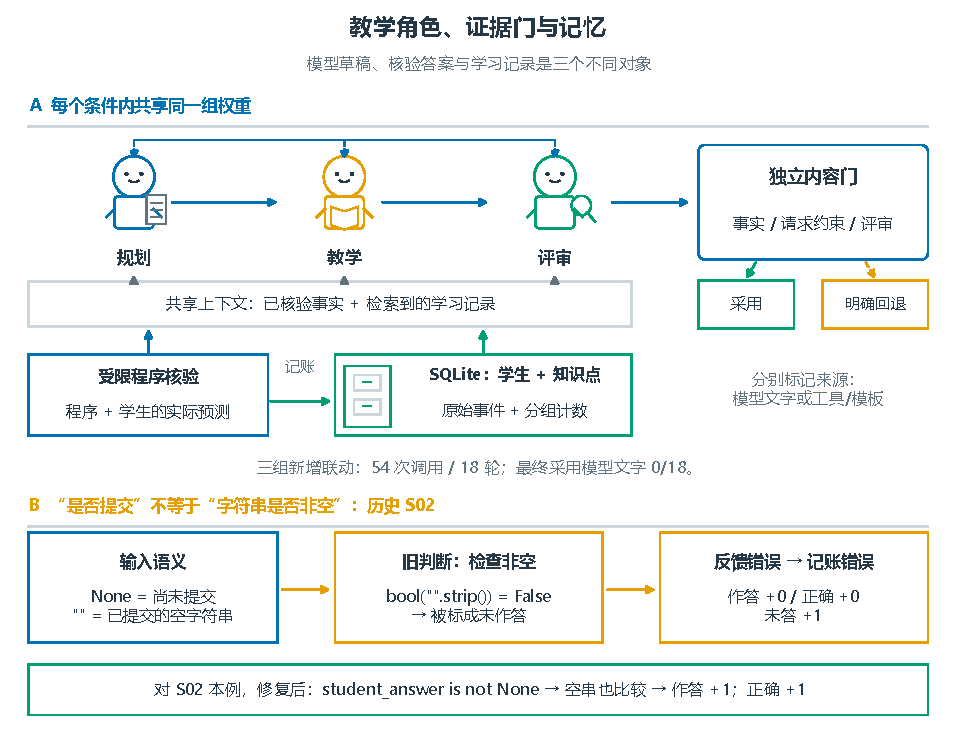
\includegraphics[width=\linewidth]{../../assets/zh/teaching-memory.pdf}
\caption{共享模型、角色调用、独立核验与学生记忆。历史空字符串故障与后续修复分开标记；角色形象只解释职责，不代表独立训练的模型。}\label{fig:concise-agents-system}
\end{figure}\FloatBarrier

SQLite 保存原始事件和派生统计。事件包括学生标识、主题、程序、预测、证据、角色输出及最终回答；统计区分交互、作答、正确、错误、未答和未核验。两层在同一事务中写入，重复事件编号不能再次计数；模型答案不算学生作答。对学生 $u$、主题 $k$、结构难度 $d$，令 $v_t$ 表示执行已核验，$a_t$ 表示已提交预测，$z_t$ 表示预测与核验输出一致，则
\begin{equation}
N_{u,k,d}\leftarrow N_{u,k,d}+v_ta_t,\qquad
C_{u,k,d}\leftarrow C_{u,k,d}+v_ta_tz_t.
\end{equation}
这些是描述统计，不是校准后的掌握概率。原版以非空文本近似 $a_t$，其问题由 S02 实测揭示。

检索按调用者提供的学生ID与主题匹配，读入最近三条事件；这以可信调用者为前提，ID过滤不等于身份认证。重建系统对象后仍读取同一数据库。难度建议从最近100条相关事件中提取同一结构难度的可核验预测，并纳入本轮：连续三次正确建议升级，连续两次错误建议降级，其余保持；实际交付题目是否更难另行检查。显式主题键、受限语法和未校准阈值限制了个性化，尚未实现同义词、前置知识依赖和遗忘推理。

\section{历史协议与四个完整案例}
原批次在运行前冻结8个场景、11轮；观察后再冻结追加4个场景、6轮。参考包含原批22段、追加12段程序及变式，均独立执行。完整成功要求全部必要自动检查与全部预设定性条目通过。Codex 技术审阅保留原文依据，不属于教师盲评。追加设计者未读实现，但已看原案例与结果，因而属于定向覆盖扩展，不是随机样本或全程外部盲测。

两批共12个场景，7项完整、5项未完整，自动检查145/150；51次真实角色调用均未采用，17轮最终回答全部来自工具和模板。C03/C04 超过各自事前“部分完成”预期；C08/S02 低于各自运行前“完整完成”预期。C07 始终是预期内限制，没有为了凑数改标。C03 冻结理由曾提及此前“range/配对误答”，但 训练研究 未实际测试 range 生成；该措辞仅保留为跨概念风险推测，不作为已观察的先前 range 故障。

\begin{figure}[htbp]\centering
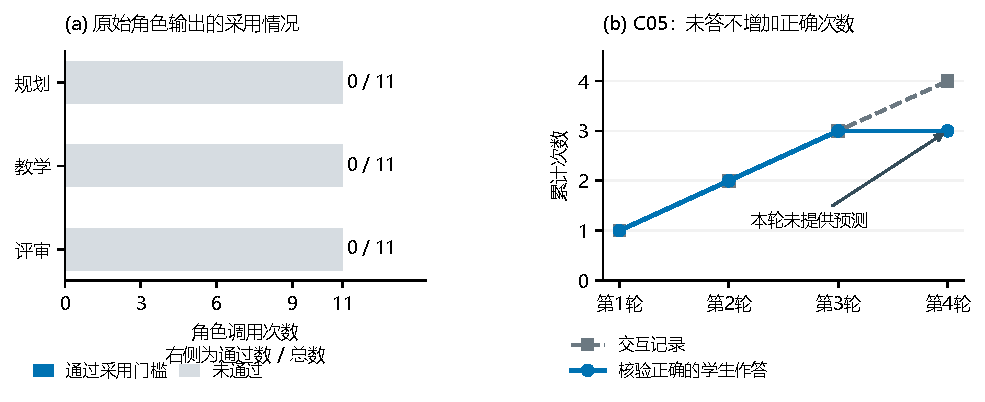
\includegraphics[width=\linewidth]{../../assets/zh/agents-evidence.pdf}
\caption{历史观测：原批11轮中角色输出采用均为零；C05 第四次交互未提交预测，因此正确作答数保持为3。自动记账与教学任务完整性是不同指标。}\label{fig:concise-agents-evidence}
\end{figure}\FloatBarrier

以下保留实际中文回答摘录。完整题目、参考、角色原文、最终回答及散列见 \path{tutor/legacy/results/core/}、\path{tutor/legacy/results/supplement/}；四案例的原文与英文完整译文还见 \path{reports/case-study-evidence.en.json}。

\Needspace{18\baselineskip}
\subsection{C03：跨实例取回旧错因}
\paragraph{任务与参考。}
学生此前把 \texttt{range(2,8,2)} 的终点8计入，预测20而非12。本轮重建系统对象后，预测下列程序为9，要求联系旧错误反馈，并提供给定的同概念复测：
\begin{verbatim}
total = 0
for n in range(3, 9, 3):
    total += n
print(total)
\end{verbatim}
正确结果为 $3+6=9$，终点9排除；给定复测将终点改为12，得到 $3+6+9=18$。

\Needspace{15\baselineskip}
\paragraph{实际回答与解释。}
原始教师反复生成核对错因的指示，未形成合格结构化回答，被拒绝。最终回答摘录为：
\begin{quote}\small
上次同一概念的记录中，你的预测与实际输出不一致。你写的预测是 '20'，核验输出为 '12'。当时你的原话是「我把 8 也加进去了，所以猜 20」。这只是作答证据，不等于掌握结论。

本题输出：9

你的这次预测与程序实际输出一致。

第 2 行（主程序）：range(3, 9, 3) 实际取值 [3, 6]；终点 9 不包含在内。

复测参考输出：18
\end{quote}
数据库保留两次预测、一对一错。检索跨对象重建仍有效，并保留旧证据，超过事前部分完成预期；引用来自确定性数据库读取，解释来自执行轨迹，不是已证明的模型学习者推理。

\Needspace{17\baselineskip}
\subsection{C04：同主题下隔离新学生}
\paragraph{任务与参考。}
另一名学生没有提交预测，请求解释下列程序并交付给定复测，不能继承上一名学生的经历：
\begin{verbatim}
total = 0
for n in range(2, 8, 2):
    total += n
print(total)
\end{verbatim}
原题为 $2+4+6=12$；给定复测将终点改为10，得到 $2+4+6+8=20$。作答数和正确数均应保持零。

\Needspace{13\baselineskip}
\paragraph{实际回答与解释。}
原始教师反复列出提取执行步骤、生成复测片段的指示，没有可用回答。最终工具和模板反馈为：
\begin{quote}\small
本题输出：12

这次未提供预测，因此不记录为作答正确或错误。

第 2 行（主程序）：range(2, 8, 2) 实际取值 [2, 4, 6]；终点 8 不包含在内。

复测参考输出：20
\end{quote}
检索结果为空，写入后该学生交互1次、作答0次、未答1次；没有引用旧学生错因，超过部分完成预期。这验证本次身份隔离，不证明系统能深度适应不同学习背景。

\Needspace{21\baselineskip}
\subsection{C08：执行正确，但变式违反修改约束}
\paragraph{任务与参考。}
学生预测230，要求列出各对贡献、未配对尾项，并且\emph{只在右列表末尾追加一个数}形成复测。原题与实际交付代码并列如下：
\par\noindent\begin{minipage}[t]{0.48\linewidth}\small
\textbf{原题程序}\par
\begin{verbatim}
left = [9,24,17,32,6,18]
right = [7,16,35,22,44]
total = 0
for a, b in zip(left, right):
    total += a + b
print(total)
\end{verbatim}
\end{minipage}\hfill
\begin{minipage}[t]{0.48\linewidth}\small
\textbf{实际交付复测}\par
\begin{verbatim}
left = [9,24,17,32,6,18]
right = [7,16,35,22,44]
total = 1
for a, b in zip(left, right):
    total += a + b
print(total)
\end{verbatim}
\end{minipage}\par
五对贡献为 $16,40,52,54,50$，合计212；左侧末尾18无配对。参考在右侧追加6，得到 $212+18+6=236$；其他追加值也可合法，只需代码和解释一致。

\Needspace{8\baselineskip}
\paragraph{实际回答与根因。}
不合格的原始教师回应被拒。最终回答正确给出212及逐对贡献，却又交付：
\begin{quote}\small
复测题：只把原第 3 行的 0 改为 1，其余不变。

复测参考输出：213
\end{quote}
代码确实输出213，但改的是累加初值，右列表未增长，仍只有五对。原有5项自动检查全部通过；缺失的是修改是否符合教学请求，而不是能否运行。该案例低于事前完整完成预期，是原批真正的意外失败。

\Needspace{20\baselineskip}
\subsection{S02：正确空字符串预测被当作未答}
\paragraph{任务与参考。}
学生显式提交 \texttt{student\_answer=""}，原话为“我的预测是空字符串，也就是只打印一个空行”。原题与给定复测为：
\begin{verbatim}
word = 'python'
print(word[4:1])   # Original
word = 'python'
print(word[1:4])   # Supplied follow-up
\end{verbatim}
默认正步长使 \texttt{[4:1]} 选不到下标。CPython 原始输出恰为一个换行，归一化后为空字符串，与预测一致；作答和正确应各加1，未答不变。复测参考为 \texttt{yth}。

\Needspace{12\baselineskip}
\paragraph{实际回答与根因。}
原始教师误称原切片返回 \texttt{python}，被拒绝。最终回答的输出字段确实为空：
\begin{quote}\small
本题输出：

这次未提供预测，因此不记录为作答正确或错误。

第 2 行（主程序）：word[4:1] 取下标 []，得到 \texttt{''}。

复测参考输出：yth
\end{quote}
不能在第一行冒号后补写系统未曾说出的“空字符串”。执行与复测正确，反馈和 SQLite 却将显式预测标为 \texttt{unanswered}：作答与正确保持零、未答增加1，自动检查仅5/9。\texttt{bool(student\_answer.strip())} 在比较答案前将有效空内容合并为未提交。这是不同于 C08 的状态表示故障，低于追加批运行前的完整完成预期，补齐第二个真正意外失败，无需更改 C07 标签。

\begin{figure}[htbp]\centering
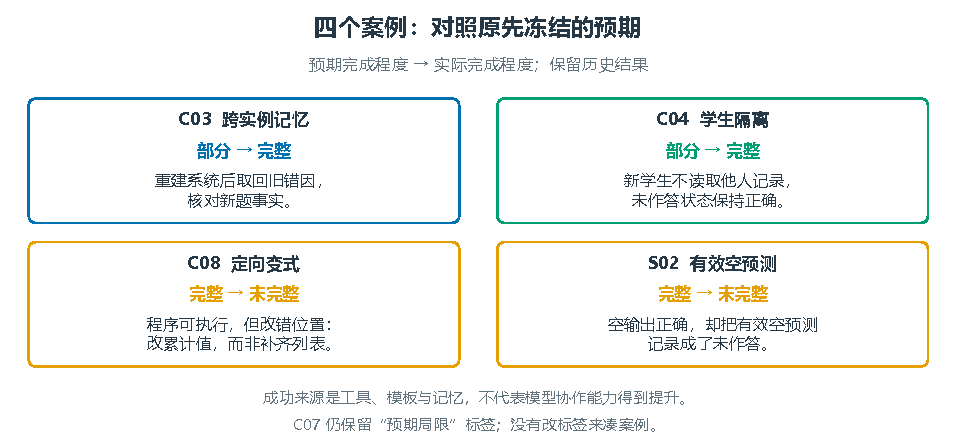
\includegraphics[width=\linewidth]{../../assets/zh/case-outcomes.pdf}
\caption{四个历史案例与各自运行前预期。C03/C04 成功依赖已核验记录和模板；C08/S02 暴露不同控制器缺陷。后续修复不抹去原结果，也不将历史失败改成新成功。}\label{fig:concise-agents-cases}
\end{figure}\FloatBarrier

\section{修复、对照与模型联动}
修复隔离在 \path{tutor/core/}，原输入、数据库、文件、预期和标签保持不变；已知案例回归不算未知测试。14项单元测试另覆盖否定、修改范围、空白输出、错误状态和身份隔离，脚本后端仅用于单元测试。

C07 的漏练习来自12字符窗口遇到16字符间隔。修订识别器去掉窗口并检查否定；受限的空列表、空字典默认值修复使用 \texttt{None} 和入口新建容器。C08 要求删去右列表新增元素后恢复原 AST，追加1输出231，是参考236之外的合法变式。S02 区分 \texttt{None} 与已提交空文本，规范化仅删末尾一次换行；修复计数为作答+1、正确+1、未答+0。首版修复工具卡把默认表达式列表 \texttt{[None]} 误当作可变默认容器，而函数实际默认参数已是 \texttt{None}；后来统一管线按类型和入口 AST 纠正。代码正确未自动保证说明正确。

\begin{table}[htbp]\centering\small
\caption{控制器与记忆对照。采用模型文字不等于教学质量达标。}\label{tab:concise-agents-controls}
\begin{tabularx}{\linewidth}{@{}Yrrrr@{}}\toprule
配置 & 轮数 & 调用 & 最终采用 & 检查\\\midrule
工具模板，开启记忆 &17&0&0&209/209\\
同系统，关闭记忆读取 &17&0&0&204/209\\
官方 Instruct，多角色 &17&51&1&209/209\\
官方 Instruct，单角色子集 &6&6&1&70/70\\\bottomrule
\end{tabularx}
\end{table}\FloatBarrier

关闭记忆仍写审计事件，但少了 C03/S03/S04 三次历史检索，以及 C05 难度建议、交付两项检查，支持这些机制在本次输入中的作用，不证明模型记忆推理或学习收益。官方 Instruct 是外部诊断，不代替自训练 SFT。17份教师原文中13份复制数值示例；17份评审全部批准，包括错误草稿。仅 C03 通过外部门槛，其采用文字逐字复述 F1 工具卡。同六题的单、多角色教师原文与最终文本相同，调用6对18次、生成耗时约35.0对73.5秒，没有观察到最终回答增益。

\begin{table}[htbp]\centering\small
\caption{相同八个新挑战上的提示与证据诊断。任务在调用前冻结但受已见故障启发；围栏兼容看过同题输出后修订，属于探索性复测。}\label{tab:concise-agents-prompt}
\begin{tabularx}{\linewidth}{@{}Yrrrr@{}}\toprule
条件 & 调用 & 教师解析 & 最终采用 & 检查\\\midrule
去示例，自由解释 &24&8/8&1/8&64/64\\
去示例，裸 JSON 严格引文 &24&0/8&0/8&64/64\\
完整围栏兼容复测 &24&8/8&1/8引文&64/64\\\bottomrule
\end{tabularx}
\end{table}\FloatBarrier

自由解释答案匹配7/8，学生状态仅2/8，唯一采用只是通用工具说明。严格组围栏内字段人工核读为答案7/8、状态3/8，但正式裸 JSON 解析仍为零。完整围栏兼容恢复结构读取，却没有修好这些状态；7次评审批准仍违反内容合约。只有 P03 采用\emph{模型选择的工具证据}，不是独立自由解释。教师原文与前严格组相同，解析使评审输入改变，因此是真实管线重跑，不能把离线解析算作新模型推理。原六题的探索性配对每条件18次调用：自由解释采用2/6，但一例从一次正确预测过度推断理解；严格引文解析和采用均为零。两组70/70来自核验与回退。提示、控制器和工具卡同时改变，不能视为纯提示消融。

\begin{figure}[htbp]\centering
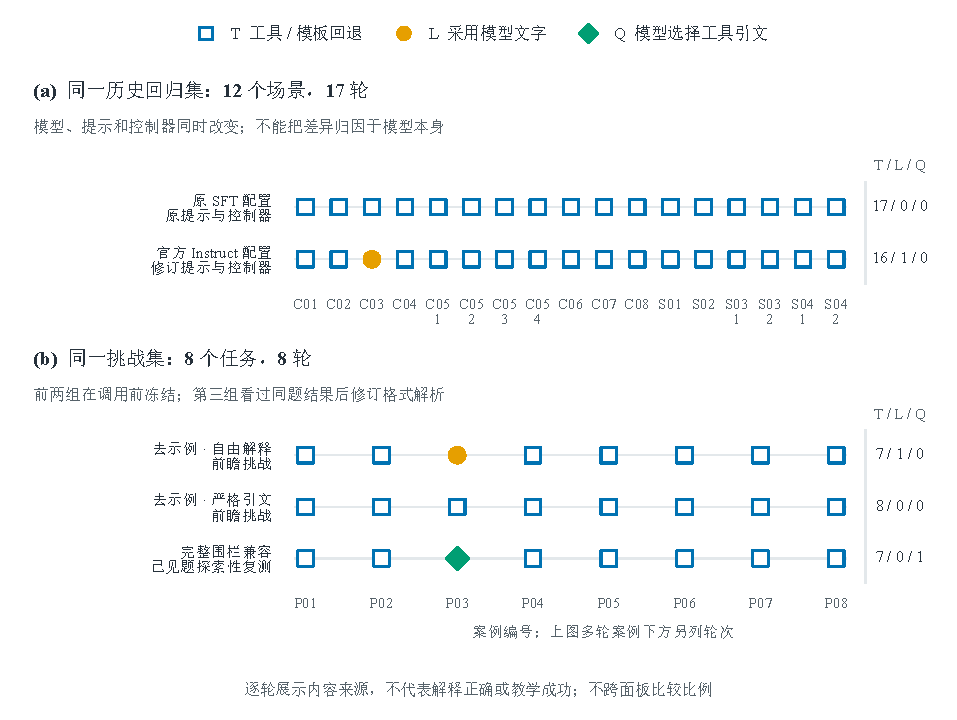
\includegraphics[width=\linewidth]{../../assets/zh/agents-revision-provenance.pdf}
\caption{实际记录的最终内容来源：工具模板、采用模型原文和模型选择工具引文。两面板任务集不同，不比较总体采用率；选择引文不证明独立推理或教学价值。}\label{fig:concise-agents-provenance}
\end{figure}\FloatBarrier

真实云端检查点另行联动：首轮 SFT 来自 首次云端运行，追加 SFT 来自 探索性追加运行。各组使用相同已知六题、64/192/96预算、本机 CPU float32 和贪心解码，未加载 DPO。Instruct 官方封装比 SFT 多21个系统开头 token；历史事件编号、规划采用和草稿也可能改变后续上下文，不能作只替换权重的因果比较。

\begin{table}[htbp]\centering\small
\caption{相同六题的四组自训练 SFT 部署。每组18次真实调用、工程检查70/70；正常结束只表示结束标记，不表示回答正确。}\label{tab:concise-agents-sft}
\begin{tabularx}{\linewidth}{@{}Yrrr@{}}\toprule
管线与检查点 & token & 正常结束 & 最终采用\\\midrule
原修复管线，首轮 SFT &2112&0/18&0/6\\
同管线，追加 SFT &1914&3/18&0/6\\
统一去示例管线，首轮 SFT &2112&0/18&0/6\\
同统一管线，追加 SFT &1895&2/18&0/6\\\bottomrule
\end{tabularx}
\end{table}\FloatBarrier

首轮云 SFT 的角色采用0/18、最终解释采用0/6；后三组新增54次真实调用、5921个 token。同一管线内，首轮和追加检查点的六份最终回答逐字相同，均使用模板。原文仍有错误答案、状态和解释，例如一边包含 range 排除终点、一边将终点求和，空输出写成9，或答案正确却批准学生错答。因此，零采用不只是 JSON 格式过严。统一管线正确的 \texttt{None} 说明来自工具卡修复，不是模型增益。散列绑定的非盲化技术审阅另存，没有回写冻结运行中的 \texttt{unreviewed} 状态。

\section{解释与证据入口}
后续输出控制复核发现，隐藏答案时也会省略用户明确请求的练习。\path{tutor/rendering/}隔离修订将题目交付与答案显示拆开，6项工具模式回归通过，未调用模型；历史案例、标签和采用率保持原记录。

本次输入支持持久记录、学生隔离和若干确定性约束有效，但未证明自主教学、多角色优越性或学生学习收益。原案例与系统共同开发，后续挑战和回归受已见故障引导；没有同管线基础模型或真实学生对照来支持训练、学习收益的因果结论。实验已经停止，成功与真实失败共同保留。

逐例评分、全部原文、token及耗时、提示变体、源码散列和修复审阅见 \path{tutor/legacy/}、\path{tutor/core/}、\path{tutor/structured/}、\path{tutor/fence/}。保留的完整报告提供展开过程；本章只合并研究阶段，不替换原记录。

\paragraph{阅读提示（不属于新实验）。}
可以把工具看作计算器，把记忆看作按学生和主题索引的笔记本，把模型看作负责组织解释的讲解者。计算正确、记住旧事和讲解可靠是三件事。本章四案例及后续对照分别检查它们，不能把“工具最终答对”当成“模型已经学会教学”。
